\section{Modeling}
\label{method}
In this section, we present the modeling strategies of \textbf{MiniOneRec}, as illustrated in Figure \ref{fig:framework}. 
MiniOneRec first convert the textual information into semantic IDs with RQ-VAE tokenizer (Section \ref{sec:tokenization}). 
For better incorporating the huge world knowledge within LLMs \citep{LlaRA}, MiniOneRec further introduce the alignment with LLMs as one expansion of the original OneRec architecture (Section \ref{sec:alignment_llm}). 
During the training stage, MiniOneRec is optimized with next token prediction first, and then followed by reinforeced preference optimization (Section \ref{sec:optimization}). 



\slh{
\begin{figure}
    \centering
    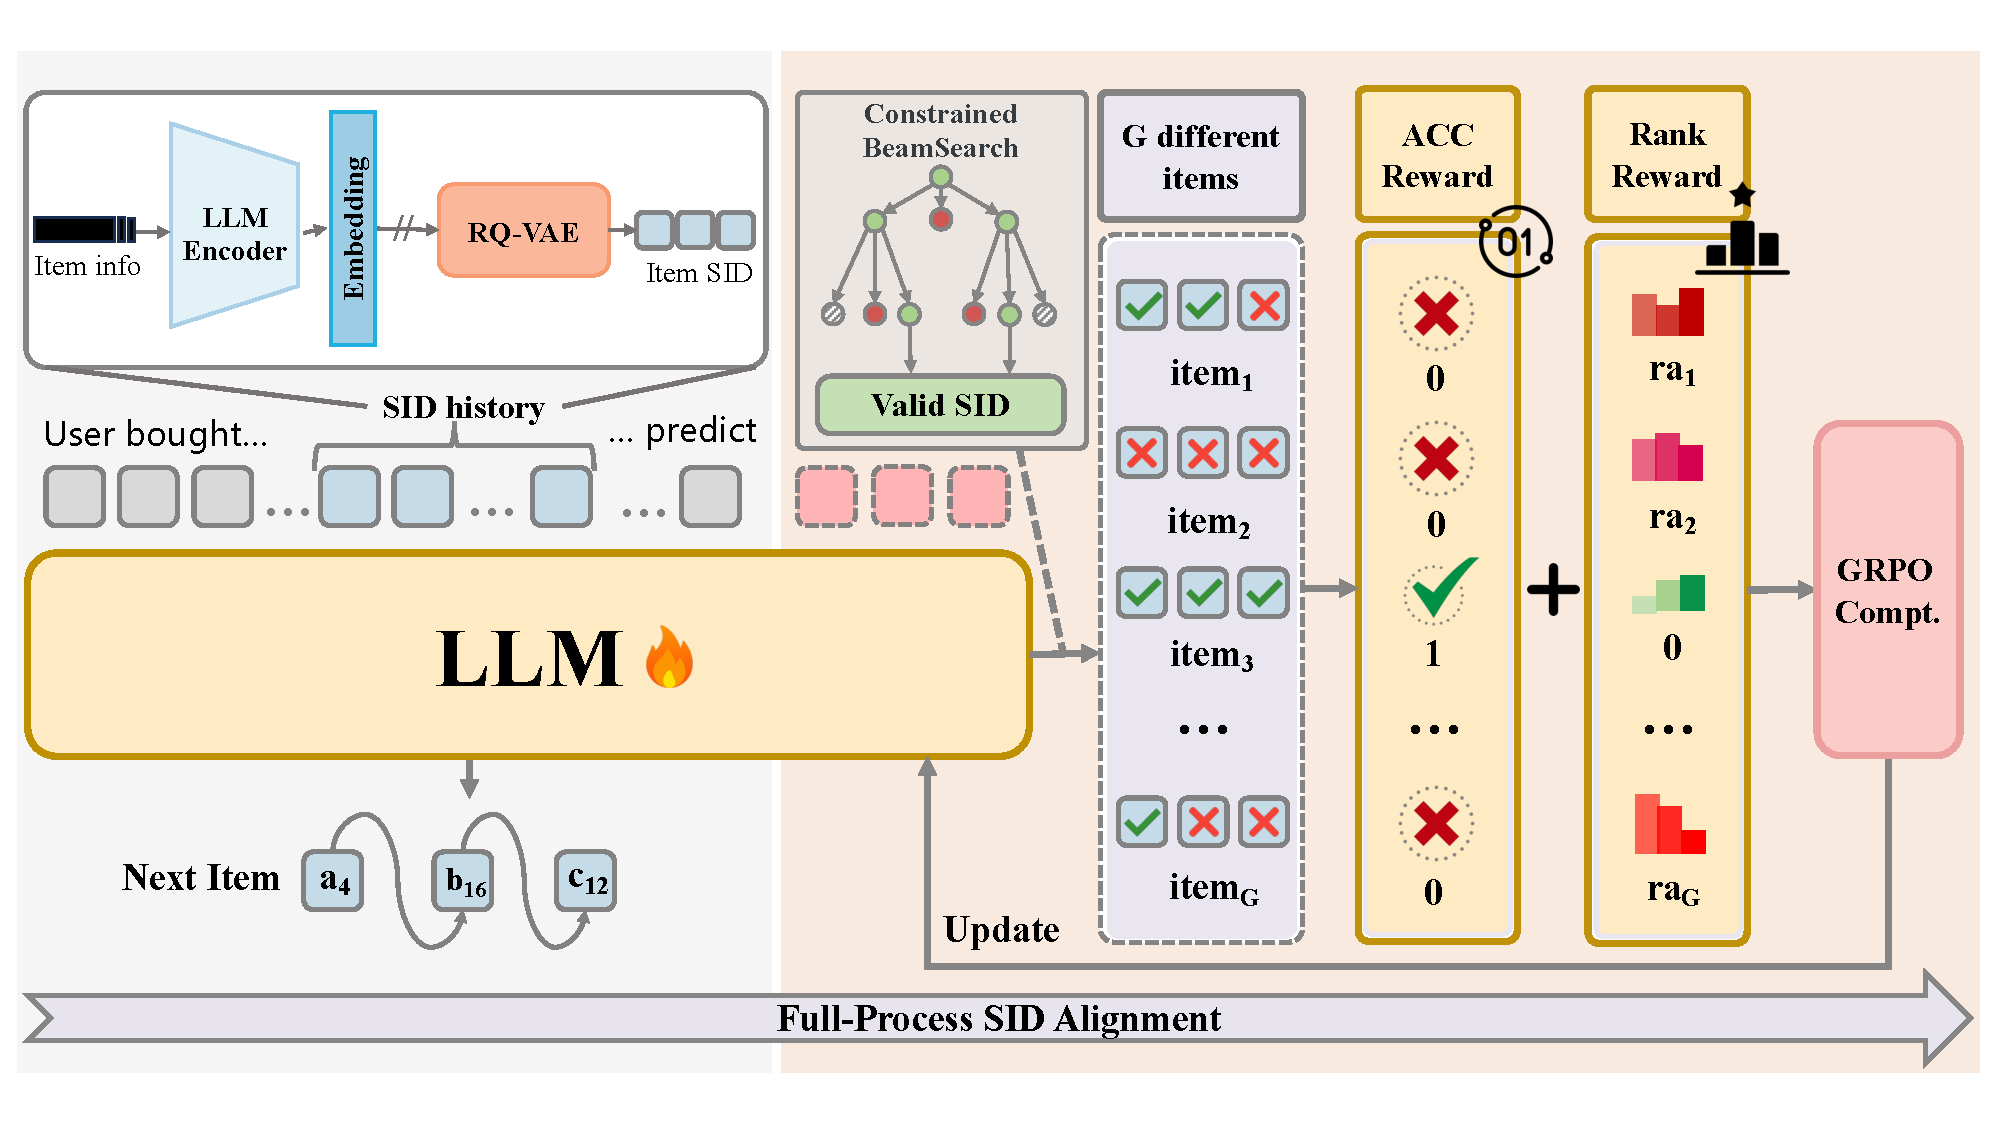
\includegraphics[width=0.85\textwidth]{figures/MiniOneRec_framework.pdf}
    \vspace{-10pt}
    \caption{MiniOneRec framework. RQ-VAE builds the item SID codebook. We then perform SFT to warm up the LLM and obtain an initial alignment. In RL, beam search with constrained decoding, thereby the model sequentially produces a ranked list of distinct, valid SIDs. GRPO updates the policy, and SID alignment is enforced end-to-end. This alignment objective is preserved throughout both the SFT and RL stages, fostering deeper semantic understanding.}
    \label{fig:framework}
    \vspace{-10pt}
\end{figure}

% To address the key shortcomings of the existing SFT-then-RL pipeline for generative recommendation, we propose \textbf{MiniOneRec}.  
% The framework elevates the performance ceiling by aligning the LLM with the SID space throughout the entire training process and applying preference optimization in the RL stage, as illustrated in Figure \ref{fig:framework}.

\subsection{Task formulation}
Generative recommendation reformulates the recommendation problem as a sequence generation task.
% where an autoregressive sequence model is trained to output a series of item identifiers that constitute personalized recommendations.
Let $H_u$ denote the interaction history of user $u$, sorted in chronological order.  
Each item $i \in H_u$ is represented by a $3$–level SID tuple $\{s^{(1)}_{i},\,s^{(2)}_{i},\,s^{(3)}_{i}\}$.  
Given $H_u$, the generative recommender $\pi_{\theta}$, parameterized by $\theta$, is trained to predict an item $i^{\text{pos}}$ that best matches the preferences of user $u$ from the item set.  
During inference, we employ beam search to generate the top-$k$ candidates and evaluate the model with standard generative-recommendation metrics.

\slh{
\subsection{Item Tokenization} \label{sec:tokenization}

% \begin{equation}
    %L_{RECON} = ||e-\hat{e}||_{2}^{2}
% \end{equation}

% \begin{equation}
% \mathcal{L}_{\mathrm{RQ}}=\sum_{i=0}^{m-1}\left\|\operatorname{sg}\left[\boldsymbol{r}_{i}\right]-\boldsymbol{e}_{c_{i}}^{i}\right\|_{2}^{2}+\beta\left\|\boldsymbol{r}_{i}-\operatorname{sg}\left[\boldsymbol{e}_{c_{i}}^{i}\right]\right\|_{2}^{2},
% \end{equation}

% \begin{equation}
% L_{rq-vae} = L_{RECON} + L_{RQ}
% \end{equation}

Following the standard item tokenization pipeline in SID-based generative recommender systems, such as TIGER \citep{TIGER} and OneRec \citep{OneRec}, we adopt RQ-VAE \citep{rqvae} as the item tokenization method. }
For each item $i$, we concatenate its title and textual description and feed the resulting sentence into a frozen content encoder to produce a $d$-dimensional semantic vector $\mathbf{x}\in\mathbb{R}^{d}$.
% $\mathbf{x}\in\mathbb{R}^{d}$.
RQ-VAE then performs residual quantization on $\mathbf{x}$ to produce a sequence of codewords.

\subsection{Alignment with LLMs} \label{sec:alignment_llm}
As demonstrated in Section~\ref{llmmatter}, aligning world knowledge with item SIDs is beneficial for generative recommendation.  
Hence, instead of the original paradigm in OneRec that trains only on SIDs \citep{TIGER, OneRec, mtgr}, our LLM-based recommender explicitly strengthens the link between language understanding and collaborative semantics by injecting a set of alignment objectives:
\begin{itemize}[leftmargin=*]
    \item \textbf{Semantic Tasks.} 
    Given a chronologically ordered sequence of historical SIDs and an explicit task instruction, the LLM is asked to predict the SID of the next item the user is likely to interact with. 
    \item \textbf{Alignment Tasks.} % Bridging tasks that transfer knowledge between the semantic and textual spaces. 
It comprises a series of alignment tasks between the textual space and the SID space. Through these tasks, we encourage a bidirectional mapping that grounds SIDs in language and injects linguistic knowledge into SID representations.
\end{itemize}
Representative tasks from each category are jointly optimized throughout the entire SFT-then-RL pipeline, enabling the LLM to fully exploit its world knowledge, deepen its understanding of SIDs, and ultimately boost generative-recommendation performance. During the RL phase, we employ constrained decoding, limiting the output space to a precompiled dictionary that contains the SID of each item as well as its canonical title. This restriction ensures that the LLM can emit only legal identifiers, making it straightforward to compute a rule-based, verifiable reward signal. Detailed examples of the prompts are provided in the Appendix \ref{appendix:align_prompt}.
}

\subsection{Reinforced Preference Optimization} \label{sec:optimization}
We fine-tune our policy with the GRPO algorithm \citep{deepseekmath,deepseek}, which leverages the relative quality of multiple responses generated for the same prompt. Concretely, for each input $x\!\sim\!D$, we roll out the current policy $\pi_{\theta_{\text{old}}}$ $G$ times to obtain a set of candidates $\mathcal{Y}(x)=\{y^{(1)},\dots,y^{(G)}\}$.  Each candidate $y^{(i)}$ receives a scalar reward $R_i$, and the advantage is computed by normalizing the rewards \emph{within the group}
\begin{equation}
    \hat{A}_i=\frac{R_i-\operatorname{mean}(R_{1:G})}{\operatorname{std}(R_{1:G})},
    \label{eq:grpo_adv}
\end{equation}
where $R_{1:G}=\{R_1,\dots,R_G\}$. This groupwise normalization recenters advantages at zero and rescales them to unit variance, thereby turning each prompt into a self-contained comparison game and reducing gradient variance.  The new policy $\pi_\theta$ maximizes the clipped surrogate
\begin{equation}
\begin{aligned}
J_{\text{GRPO}}(\theta)=\;
&\mathbb{E}_{x\sim D,\; y^{(i)}\sim\pi_{\theta_{\text{old}}}}
\Biggl[
\frac{1}{G}\sum_{i=1}^{G}\frac{1}{|y^{(i)}|}
\sum_{t=1}^{|y^{(i)}|}
\Bigl\{
\min\!\bigl(r_{i,t}\hat{A}_{i,t},\,
\operatorname{clip}(r_{i,t},1-\epsilon,1+\epsilon)\hat{A}_{i,t}\bigr)
\\[4pt]
&\qquad
-\beta\,\mathrm{KL}\!\bigl[\pi_\theta\|\pi_{\text{ref}}\bigr]
\Bigr\}
\Biggr],
\end{aligned}
\label{eq:grpo_obj}
\end{equation}
where 
$r_{i,t}=
\tfrac{\pi_\theta(y^{(i)}_t\,|\,x,y^{(i)}_{<t})}
      {\pi_{\theta_{\text{old}}}(y^{(i)}_t\,|\,x,y^{(i)}_{<t})}$
is the per-token importance ratio, $\epsilon$ is the clipping threshold, and $\beta$ balances task reward against a KL penalty, keeping the updated policy close to a reference model $\pi_{\text{ref}}$.

\slh{
Adapting Reinforcement learning with verifiable rewards (RLVR) to recommendation is not straightforward, as it raises two key challenges in sampling and reward design.
First, unlike open-ended language generation, the output space of recommendation is constrained to valid item SIDs. 
It is much narrower and makes repeated sampling from the same prompt prone to severe duplication, which in turn leads to low sampling efficiency. 
To mitigate this, we incorporate dynamic sampling \citep{DAPO} and constrained beam search to improve sampling efficiency and expose the model to more informative negative items.

On the other hand, while ranking ability is essential for recommendation, the rule-based reward assigns zero to all negatives, providing only coarse-grained feedback. 
This exposes a broader challenge: reward design in recommendation remains under-explored, yet holds significant potential for richer supervision. 
To move beyond binary correctness, we propose an auxiliary ranking reward that penalizes harder negatives with lower scores, and further investigate the potential of dense rewards such as semantic and collaborative signals.

\subsubsection{Sampling Strategy}
\label{subsection:sampling}
A key challenge in adapting RLVR to recommendation lies in the low sampling efficiency caused by the narrow item space: repeatedly sampling from the same prompt often yields duplicate items, reducing the diversity of sampled negatives. 
To quantify this, we define generation diversity as
\begin{align}
    \label{eq:diversity}
    \text{div}(\{e_k\}_{k=1}^G)=\frac{\text{uni}(\{e_k\}_{k=1}^G)}{G},
\end{align}
where $\text{uni}(\{e_k\}_{k=1}^G)$ counts the number of unique items among $G$ generations. 
Higher diversity exposes the model to richer negative signals and thus improves ranking supervision.
To enhance sampling efficiency, we explore two complementary strategies.
We first explore dynamic sampling, which over-generates candidates and then selects a subset that balances inclusion of the target item with maximizing negative diversity. 
However, this strategy requires generating substantially more samples, and its diversity also inevitably declines as training progresses. 
Motivated by these limitations, we ultimately adopt beam search as our sampling method. 
Beam search ensures that all sampled items are distinct, thereby improving efficiency and diversity. 
Following \citep{Decodingmatters}, we remove length normalization to avoid amplification bias.

\subsubsection{Reward Design}
% \label{method:reward}
Recommendation quality is usually measured by ranking metrics like NDCG, highlighting the importance of fine-grained ranking ability. 
However, the rule-based reward in GRPO only distinguishes the target item from all others, assigning $1$ to the positive and $0$ to every negative.
This implicitly assumes that all negatives contribute equally during optimization and only injects coarse-grained ranking information into LLMs.
% To further corroborate our analysis, we provide a gradient study of GRPO in Appendix \ref{Appendix:gradient}.

% assigning larger gradients to hard negatives 
Prior works have shown that emphasizing hard negatives improves the discriminative ability of recommendation models \citep{SGL, sdpo}.
Motivated by this insight, we introduce a ranking reward penalizing harder negatives more heavily. 
Specifically, for a generated negative item $e_k$, we compute its generation rank $\rho_k$ and assign a lower reward to negatives with higher-probability:
\begin{align}
    \hat{R}_\text{rank}(e_k, e_t)=\begin{cases} 
    0, & e_k=e_t \\
    -\frac{1}{\log(\rho_k+1)}, & \text{otherwise} 
    \end{cases},\\
    R_\text{rank}(e_k,e_t)=-\frac{\hat{R}_\text{rank}(e_k,e_t)}{\sum_{j=1}^G \hat{R}_\text{rank}(e_j,e_t)}. \label{eq:ranking_reward}
\end{align}
Finally, the overall reward combines the standard rule-based reward and the ranking reward:
\begin{align}
    R(e_k,e_t)=R_\text{rule}(e_k,e_t)+R_\text{rank}(e_k,e_t).
\end{align}
This combined reward integrates binary correctness with ranking signals, providing richer supervision that enhances the model’s ability to discriminate among negatives and improves ranking performance.
While the ranking reward provides finer-grained supervision than the binary rule-based reward, reward design in recommendation remains largely under-explored. 
}


